\documentclass[11pt]{article}
\usepackage[margin=1.1in]{geometry}
\usepackage{amsmath,amssymb}
\usepackage{booktabs}
\usepackage{array}
\usepackage{tabularx}
\usepackage[protrusion=true,expansion=false]{microtype}
\usepackage[table]{xcolor}
\usepackage{enumitem}
\usepackage{tikz}
\usepackage{float}
\usetikzlibrary{arrows.meta}
\usepackage{hyperref}

\hypersetup{pdftitle={Licash: owner-bound ecash with local Bitcoin recovery}, colorlinks=true, linkcolor=blue!60!black, urlcolor=blue!60!black, citecolor=blue!60!black}
\usepackage[skip=0.6\baselineskip, indent=0pt]{parskip}

\makeatletter
\renewcommand\section{\@startsection{section}{1}{\z@}{-2.5ex plus -1ex minus -.2ex}{1.2ex plus .2ex}{\large\bfseries}}
\renewcommand\@seccntformat[1]{\csname the#1\endcsname.\hspace{0.7em}}
\makeatother

\newcommand{\paperversion}{0.4}

\newcommand{\vmax}{V_{\max}}
\newcommand{\wH}{w_H}
\newcommand{\tx}[1]{\texttt{#1}}
\newcommand{\Ht}[1]{H_{\mathsf{#1}}}
\newcommand{\htc}{\mathsf{h2c}}
\newcommand{\id}{\mathsf{id}}
\newcommand{\bcorr}{b_{\mathrm{corr}}}
\newcommand{\DLEQ}{\mathsf{DLEQ}}
\newcommand{\Sign}{\mathsf{Sign}}
\newcommand{\Kiss}{K_{\mathrm{iss}}}
\newcommand{\kiss}{k_{\mathrm{iss}}}
\newcommand{\G}{\mathcal{G}}
\newcommand{\prop}[1]{\paragraph{Property #1.}}
\newcolumntype{L}{>{\raggedright\arraybackslash}X}
\renewcommand{\arraystretch}{1.3}

\definecolor{coop}{RGB}{232,245,233}
\definecolor{hubc}{RGB}{255,243,214}

\title{\textbf{Licash}\\owner-bound ecash with local Bitcoin recovery}
\author{m0wer \and waxwing}
\date{Version \paperversion, November 2026}

\begin{document}
\maketitle

\begin{abstract}
Licash is ecash in which every holder has an individual, collateralized right to recover their notes on Bitcoin from the issuer, the \emph{hub}. Payments are offchain reissuances between owner keys. They are immediate, use no blockspace and leave no public trace, and the hub cannot link the spending of a note to its issuance. A holder recovers by claiming their own notes on Bitcoin. The hub can reduce a claim only by exhibiting a spend that the holder authorized, and a claim made from a stale backup is paid exactly its unspent part. Payments are atomic without trust: the payee's notes are issued in advance under a one-time pad, and the hub must publish the pad's key on Bitcoin to retire the payer's inputs. Either the payer recovers her inputs, or the payee is paid and the payer receives her change. The same rule, publish the secret or pay the refund, yields hash-locked payments that connect a hub to onchain Bitcoin, to Lightning and to other hubs. We specify the protocol, argue its security and privacy properties, and report an implementation in which every outcome, including swaps, Lightning payments and routes across three hubs, is carried out with Bitcoin transactions.
\end{abstract}

\section{Introduction}

Licash comes from lichen ecash and is pronounced ``lee cash.''

Bitcoin payments are public and compete for blockspace. Receiving to fresh addresses does not help once the coins are spent together, because consolidation links its inputs. Our goal is to move routine payments and the merging of value offchain, so that they are private, cheap and fast, while every user keeps the ability to recover their money on Bitcoin without anyone's cooperation.

Ecash~\cite{chaum,cashu,fedimint} is private and cheap, but custodial: users trust the mint with their money. Designs with unilateral exit usually judge an exit against shared state, such as a state root, a transaction tree~\cite{ark}, or nullifiers reconstructed from Bitcoin~\cite{shieldedcsv,shieldedbitcoin}. That history must be ordered and available to everyone. Lichen~\cite{lichen} instead gives each user a bilateral Bitcoin contract with an operator, and in its BABE variant~\cite{babe} a dispute verifies a Groth16 proof through the contract's transaction graph.

Licash uses such contracts to back \emph{owner-bound ecash}. A payment reissues value to keys that only the recipient controls, without naming any contract. A holder recovers through the contract registered under their own spending identity, never through another user's. Instead of proving absence from a global spent set, the holder proves that their notes were issued and are theirs, and the hub must exhibit an authorized spend to reduce the claim. Recovery is therefore local: its witness concerns only the holder's notes.

Paying for something offchain is a fair exchange, which is impossible without a trusted third party~\cite{fairexchange}. As in~\cite{andrychowicz,bentov}, that party is Bitcoin, and it is used only in a dispute. The recovery rule turns the usual swap intuition around. The hub must release a secret to \emph{prevent} the payer from recovering her inputs, and that secret is what pays the payee and returns the payer's change.

A payment system is only useful if value can enter and leave it. A single mechanism, a note spend locked under a hash with an expiry, connects a hub to onchain Bitcoin, to the Lightning network and to other hubs, with the same guarantee: each party either learns the secret from Bitcoin or is refunded.

\textbf{Contributions.}
\begin{itemize}[leftmargin=1.5em, itemsep=0pt]
\item \emph{Owner-bound notes with local recovery.} A claim lists the holder's own notes, the hub answers with a proof of which of them were spent, and the contract pays the rest (Sections~\ref{sec:model} and~\ref{sec:rec}).
\item \emph{Grants.} The payee's notes are sealed under a hash pad whose key must be published to counter the payer, which makes an offchain payment atomic. Their security reduces to that of ordinary blind issuance (Section~\ref{sec:pay}).
\item \emph{Timed locks.} Hash-locked payments with forced publication of the preimage and onchain activation give swaps, Lightning payments in both directions and routes across hubs, with one deadline rule (Section~\ref{sec:interop}).
\item \emph{Unlinking.} A blinded proof of correct issuance removes the link between a note's issuance and its spending, with perfect blindness (Section~\ref{sec:model}).
\item \emph{Security, privacy and implementation.} We state and argue the properties of the protocol (Sections~\ref{sec:security} and~\ref{sec:privacy}) and evaluate a complete implementation on Bitcoin transactions (Section~\ref{sec:impl}).
\end{itemize}

\section{Model}
\label{sec:model}

\paragraph{Parties and assumptions.} The hub issues notes and funds the collateral of every contract. It may refuse service, withhold answers, issue notes it should not, collude with users or disappear. Users may double spend, claim notes they have spent and collude with each other. We assume that the discrete logarithm problem is hard in secp256k1, and that so is the one-more gap Diffie-Hellman problem~\cite{jkk,privacypass}, also against an adversary who runs the interactive Chaum-Pedersen protocol with the hub, with challenges of its choice, on points whose evaluation it has already received, that tagged hashes (including hash-to-curve) are random oracles, that BIP340 signatures are unforgeable~\cite{bip340}, that the zkVM and its Groth16 wrapper are knowledge sound~\cite{risc0,groth16}, and that BABE is sound~\cite{babe,lichenbuilt}. No party can produce in private, within the lifetime of a contract, as many valid Bitcoin blocks as the confirmation depth that the contract requires. A party that must act on Bitcoin by a deadline can get a transaction confirmed within a known number of blocks, and each party keeps its own records.

\paragraph{Notation.} $G$ is the secp256k1 generator; lowercase scalars multiply uppercase points. A denomination $d$, a power of two in satoshis, selects the hub's secret key $k_d$ with public key $K_d=k_dG$. $\DLEQ(G,K;B,C)$ is a Chaum-Pedersen proof~\cite{chaumpedersen} that $K=kG$ and $C=kB$ for the same $k$. $H_{\mathsf{tag}}$ are tagged hashes, and $\htc$ hashes a message to a curve point with the secp256k1 suite of RFC~9380~\cite{rfc9380}. A separate issuer key $\Kiss=\kiss G$ signs grants and certificates.

\paragraph{Notes.} As in Cashu~\cite{cashu}, a note is a message $x$ with a point $C=k_dY$, where $Y=\htc(x)$ is the note's \emph{identifier}. To issue it, the holder sends $B=Y+rG$ for a random $r$, the hub returns $C'=k_dB$ with $\DLEQ(G,K_d;B,C')$, and the holder computes $C=C'-rK_d$. A note is \emph{settled} once its holder has a proof that $C=k_dY$. The hub keeps a private log of the identifiers it has seen spent.

\paragraph{Owner keys.} A user has independent spend, scan and hold keys $b_s,b_v,b_h$. The public key $B_s$ is their \emph{spending root} and $(B_s,B_v,B_h)$ is their address. A payer picks an ephemeral key $A=aG$ and derives output $j$ as in silent payments~\cite{bip352}:
\begin{gather*}
\varsigma = \Ht{ecdh}(\mathsf{xcoord}(aB_v)),\qquad s_j = \Ht{seed}(\varsigma, j),\\
P_j = B_s + \Ht{tweak}(B_s, s_j)\,G,\qquad Q_j = B_h + \Ht{hold}(B_h,B_s,s_j)\,G,\\
x_j = (d_j, P_j, \nu_j, Q_j),\qquad B_j = \htc(x_j) + r_jG,
\end{gather*}
with the nonce $\nu_j$ and blinding $r_j$ also derived from $\varsigma$. The recipient recomputes both keys from $A$ before accepting an output. Only the recipient can sign for the \emph{owner key} $P_j$, which authorizes spending the note, and for the \emph{hold key} $Q_j$, which authorizes claiming it on Bitcoin. Change is derived the same way and is not marked as change. A spent note reveals $P_j$ but not $s_j$, so it does not reveal the spending root.

\paragraph{Unlinking.} The proof received at issuance contains $B$, so it would link a later spend to that issuance. The holder replaces it with a proof on $(Y,C)$ directly by blinding the Chaum-Pedersen protocol the way one blinds a Schnorr signature. The hub picks a nonce $w$ and sends $(R_1,R_2)=(wG,wB)$. The holder picks blinding scalars $\alpha,\beta$ and sends the blinded challenge $e$:
\[
R_1' = R_1 + \alpha G + \beta K_d,\quad R_2' = R_2 - rR_1 + \alpha Y + \beta C,\quad e' = \Ht{dleq}(R_1', R_2', K_d, C),\quad e = e' + \beta .
\]
The hub answers $s=w+ek_d$, once per nonce, and $(e',s+\alpha)$ is a valid proof of $\DLEQ(G,K_d;Y,C)$. Since $\alpha$ and $\beta$ are uniform, every completed session is equally likely to have produced any given unlinked proof: the blinding is perfect. A note carries either proof as its \emph{evidence}. If the hub refuses to unlink, the note keeps its value and its issuance-linked evidence.

\paragraph{Contracts.} A user and the hub open a contract by funding a Bitcoin output with the hub's collateral: a cap $\vmax$, the most the contract can pay, plus reserves for fees. The output is spent by a presigned transaction graph that uses BABE with signed payout amounts~\cite{lichen,lichenbuilt,delving}. The contract's terms, its \emph{base}, fix the hub's note keys, the user's spending root $B_s$, the cap, both parties' keys, every deadline, a Bitcoin checkpoint and the two proof programs of Section~\ref{sec:rec}. A digest $D$ binds the base to the prepared graph. Both parties verify $D$ before the funding transaction is signed, the user by signing it with $b_s$, which registers $B_s$ with the hub.

A contract is a recovery right, not an account. Notes are issued and spent without reference to any contract, and a settled note can be claimed in any one contract of its owner's spending root. A contract supports one recovery, of at most 32 items and at most $\vmax$. A holder's notes are \emph{protected} while they fit in their open contracts; value beyond that is held on trust until it is spent or a further contract covers it. Receiving a payment requires neither the recipient's presence nor unused capacity.

Between payments a holder does not watch the chain or refresh notes. Each contract has an expiry, and before its \emph{last safe action}, early enough to finish a dispute, the holder spends the notes, moves them under a newer contract or requests recovery. After expiry the collateral returns to the hub. The hub must be able to answer a request within its response window whenever one arrives.

\paragraph{Reading Bitcoin.} The proofs of Section~\ref{sec:rec} establish facts about Bitcoin, such as the height at which a transaction confirmed. They do so from a chain of block headers that extends the base's checkpoint and satisfies proof of work, the difficulty adjustment and the timestamp rules, together with Merkle inclusion proofs. Such a chain shows that an event is buried at the required depth in \emph{some} valid chain, which by our assumption on private blocks is Bitcoin's. The required confirmation depth and a header budget reaching the assertion deadline are part of the base.

\paragraph{Payout units and fees.} Denominations and payouts count satoshis. A payout omits the $L$ lowest bits of its amount to avoid dust, and the hub's reserve compensates: the base is accepted only if every transaction that pays the holder leaves her at least the omitted remainder and the fee ceilings beyond her own reserve. A holder who recovers $b$ therefore nets at least $b$ after fees, up to those ceilings.

\section{Payments}
\label{sec:pay}

A \emph{spend} $S$ lists input notes, blinded outputs $(B_j,d_j)$ of the same total value and the payer's ephemeral key $A$. Its identifier $\id(S)$ is a hash of all of it. A spend is authorized by a signature under the owner key of every input. When the hub accepts an authorized spend it records the inputs as spent and issues the outputs.

If the hub issued the outputs only after recording the spend, it could record Alice's signed payment and withhold Bob's notes. Alice's inputs would be spent, on evidence that she signed herself, and Bob would be unpaid. A \emph{grant} removes the gap. The hub issues every output before the payer signs, sealed under a key that it can use against the payer only by publishing it (Figure~\ref{fig:grant}).
\begin{enumerate}[leftmargin=1.8em, itemsep=0pt]
\item Alice sends the unsigned spend $S$ to the hub.
\item The hub draws a random 32-byte \emph{unlock} $t$ and computes, for every output $j$,
\[
C'_j = k_{d_j}B_j,\qquad \pi_j=\DLEQ(G,K_{d_j};B_j,C'_j),\qquad c_j = (C'_j \,\|\, \pi_j) \oplus \Ht{pad}(\id(S), t, j, d_j).
\]
The pad is expanded to the 97 bytes of $C'_j \,\|\, \pi_j$ by hashing with a counter. The hub returns the grant $\G = \big(\id(S),\ \Ht{lock}(\id(S),t),\ (d_j,B_j,c_j)_j\big)$, with the unlinking nonce commitments of the outputs and its signature under $\kiss$.
\item Alice checks that $\G$ lists her outputs and signs $\Ht{auth}(\id(S), \mathsf{com}(\G))$ with each input's owner key, where $\mathsf{com}(\G)$ is a hash of the whole grant, including the nonce commitments and the hub's signature. Her authorization is thereby valid for this grant only.
\item The hub records the authorized spend and releases $t$.
\item Alice sends $S$, $\G$ and $t$ to Bob. Anyone holding $\G$ and $t$ checks the lock hash, removes each pad, verifies $\pi_j$ under the ordinary key $K_{d_j}$ and unblinds $C_j=C'_j-r_jK_{d_j}$.
\end{enumerate}

\begin{figure}[H]
\centering
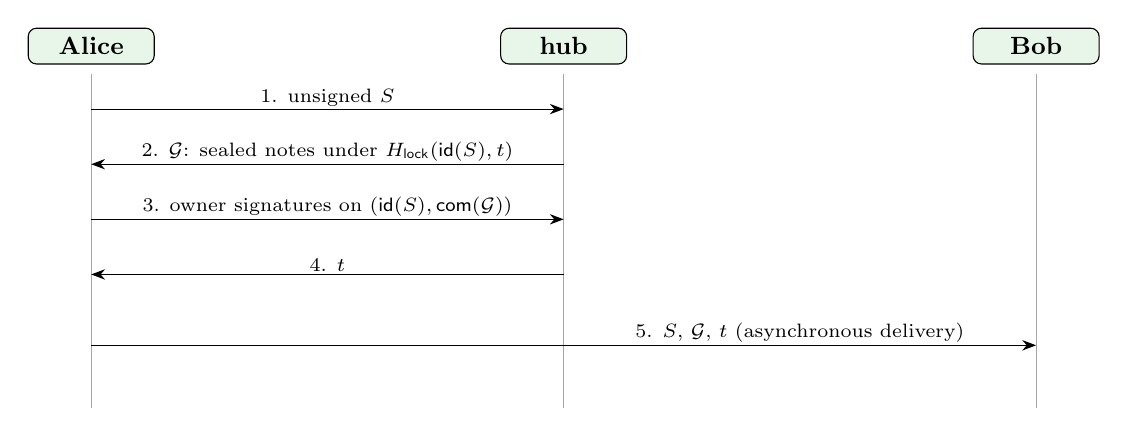
\begin{tikzpicture}[font=\small, >={Stealth[length=5pt]}, msg/.style={font=\scriptsize, fill=white, inner sep=1pt}]
\foreach \x/\n in {0/Alice, 6/hub, 12/Bob} {
  \node[draw, rounded corners=3pt, fill=coop, minimum width=16mm] at (\x,0) {\textbf{\n}};
  \draw[black!35] (\x,-0.35) -- (\x,-4.6);
}
\draw[->] (0,-0.8) -- node[msg, above] {1. unsigned $S$} (6,-0.8);
\draw[->] (6,-1.5) -- node[msg, above] {2. $\G$: sealed notes under $\Ht{lock}(\id(S),t)$} (0,-1.5);
\draw[->] (0,-2.2) -- node[msg, above] {3. owner signatures on $(\id(S), \mathsf{com}(\G))$} (6,-2.2);
\draw[->] (6,-2.9) -- node[msg, above] {4. $t$} (0,-2.9);
\draw[->] (0,-3.8) -- node[msg, above, pos=0.75] {5. $S$, $\G$, $t$ (asynchronous delivery)} (12,-3.8);
\end{tikzpicture}
\caption{A granted payment.}
\label{fig:grant}
\end{figure}

An opened note is an ordinary note with ordinary evidence, and its holder unlinks it like any other. Bob treats a payment as settled when he holds $t$ and his outputs open. Until then he has nothing, and the grant alone gives him nothing: without $t$ every $c_j$ is indistinguishable from random bytes.

Alice cannot inspect the sealed notes before she signs, and she does not need to. The hub can use her signature against her only through a counter that publishes $t$ and proves that \emph{every} sealed note of the grant opens correctly (Section~\ref{sec:rec}). A grant whose notes do not open is thus a refusal of service: the hub can never cite the spend, and Alice recovers her inputs.

Bob need not be online when Alice pays. She keeps the payment until he or his agent acknowledges it, and a mailbox or the hub can relay it. Once paid, Bob respends the notes to outputs that only he can derive and unlinks them, after which Alice no longer recognizes them.

A spend whose outputs all return to the spender, such as a consolidation or a change of denominations, needs no grant. The hub issues its outputs directly, and until it does the spender can claim them as fallbacks (Section~\ref{sec:rec}).

\section{Recovery}
\label{sec:rec}

\paragraph{Request.} A holder starts a recovery with two transactions. The \emph{request} spends the contract output and carries her one-time signatures on an amount $b$ and a claim digest $E$. The \emph{claim body} publishes the claim that $E$ commits to, in an output of at most 64,000 bytes, and must confirm within a fixed number of blocks of the request so that the hub can read it inside its response window $\wH$. A contract accepts one request.

\paragraph{Claims.} A claim lists at most 32 items of three kinds.
\begin{itemize}[leftmargin=1.5em, itemsep=0pt]
\item A \emph{settled note}, given by its message $x$.
\item A \emph{fallback}: an output of a spend that the holder signed and the hub has not answered. The claim names the spend, and all of its inputs must be among the claim's settled notes. A fallback adds nothing to $b$. It stands in for those inputs if the hub turns out to have recorded the spend.
\item An output of a \emph{timed lock} (Section~\ref{sec:interop}).
\end{itemize}
Each item carries a \emph{hold authorization}, a signature under its hold key $Q_j$ over the note's public fields, $D$, the deposit, $b$ and $E$. It binds that exact note to this contract and claim, even if another note shares its hold key. A payer who claims a timed lock on the authority of its inputs, rather than a hub certificate, authorizes its inputs in the same way and recovers that lock's outputs in one claim, never split across contracts. The amount satisfies $b \le \min(\vmax, \sum_{i\notin F} d_i)$, where $F$ is the set of fallbacks. On reading a claim the hub stops accepting spends of the claimed notes until the recovery ends.

\paragraph{The holder's proof.} The holder proves, in a zkVM program fixed by the base, that the request and the claim body confirmed on Bitcoin in time and carry her signatures on $b$ and $E$; that every settled note has valid evidence under the hub's keys; that every item's owner key derives from the base's spending root, which she shows by revealing the item's seed $s_j$ to the program; that every hold authorization verifies; and that every fallback opens an output of an authentic spend whose inputs are claimed. The proof is private: it shows nothing about her notes beyond what the claim body lists.

\paragraph{Counters.} The hub can reduce a claim only with evidence of four kinds. Against notes and fallbacks the evidence is a signature of the claimant, and against the outputs of a lock it is the resolution of that lock:
\begin{itemize}[leftmargin=1.5em, itemsep=0pt]
\item $\mathsf{Spend}(S)$: an owner-authorized spend that consumes a claimed note;
\item $\mathsf{Claim}(E')$: a hold authorization for a different claim, under the hold key of a claimed note or of an input of a claimed lock of the claimant's own notes, whose outputs it then voids;
\item $\mathsf{Preimage}(z)$ and $\mathsf{Expired}$, for the outputs of timed locks (Section~\ref{sec:interop}).
\end{itemize}
Every piece of evidence must void an item or cite the spend of a fallback. The result is a mask $M$ of voided items and a corrected amount in which the fallbacks of every cited spend take the place of its voided inputs:
\[
\bcorr = \min\Big(b,\ \sum_{i \notin M,\ i \notin F} d_i \;+ \sum_{i \in F \setminus M,\ \text{source of } i \text{ cited}} d_i\Big).
\]
The hub proves $(M,\bcorr)$ in a second zkVM program, whose public output binds $D$, $E$, the mask, the amount and a digest of the secrets disclosed below. There is no penalty. A claim made from an old backup is not fraud, and it is paid exactly the value that is still unspent: a claim of 3072 of which 1024 was spent is paid 2048. A backup protects the notes that it contains. The change of a spend made after the backup can be claimed only as a fallback of that spend, which the backup does not know, so a wallet stores every spend durably before signing it and every note when it receives it.

\paragraph{Mandatory disclosure.} A counter must not let the hub retire a payer's inputs while keeping the payee's notes sealed. A $\mathsf{Spend}$ that cites a granted spend must therefore supply the unlock $t$, and the counter program checks that $t$ matches the grant's lock and that every sealed note of the grant opens to a valid proof. Since the owners signed $\mathsf{com}(\G)$, a granted spend cannot be cited as an ungranted one. The response transaction publishes up to 32 such secrets in signed chunks whose bytes Script authenticates, and the holder's proof recomputes their digest from the bytes actually posted. A counter whose secrets were not published is no counter.

\paragraph{Response and payout.} Within $\wH$ of the request the hub signs $E$ either \emph{plainly} or with a counter: the counter proof, $\bcorr$ and the disclosed secrets. The holder then has until the assertion deadline to post a proof for one of two statements: \emph{full}, that her claim holds and the response contains no valid counter, which pays $b$; or \emph{corrected}, that her claim holds and the counter is valid, which pays $\bcorr$. BABE lets the hub challenge an assertion. A valid proof answers any challenge and is paid; an invalid one forfeits the contract to the hub. The payout is made bit by bit under the signed amount~\cite{delving}: the holder collects the set bits and the hub the clear ones.
\begin{center}
\small
\begin{tabularx}{0.95\linewidth}{LLl}
\toprule
the hub's response & the holder proves & the holder receives \\
\midrule
none within $\wH$ & nothing & $b$ \\
plain & her claim & $b$ \\
a counter that is invalid or lacks its secrets & her claim, and that the counter fails & $b$ \\
a valid counter & her claim, and that the counter holds & $\bcorr$ \\
any & nothing valid & nothing \\
\bottomrule
\end{tabularx}
\end{center}

\paragraph{Example.} Alice holds notes of 2048 and 1024. She pays Bob 512 from the first, with change of 1024 and 512, under a grant. The hub records her signed spend and withholds $t$. Alice claims both notes for 3072 and lists the two change outputs as fallbacks. If the hub does nothing she is paid 3072 and the payment never happened. To do better the hub must cite her spend, which publishes $t$: the 2048 note is voided, the change takes its place, Alice is paid $1024+1536=2560$, and Bob opens his 512 with the published $t$. The hub cannot tell an honest Alice whose answer was withheld from a dishonest Alice claiming a note she spent, and it does not need to: both are paid what they are owed.

\section{Interoperability}
\label{sec:interop}

Value enters and leaves a hub through one mechanism. A \emph{timed lock} is a spend with two sets of outputs and terms $(h, e, \delta)$: the \emph{pay} outputs are issued to the payee if a preimage $z$ of $h$ is shown before Bitcoin height $e$, and the \emph{refund} outputs are issued to the payer otherwise. Anything else that pays under the same hash, a Bitcoin HTLC~\cite{htlc}, a Lightning invoice or a lock at another hub, can then be exchanged for notes atomically. The hub signs a \emph{certificate} of each lock it accepts, binding $\id(S)$, the input identifiers and the terms. It is the hub's acknowledgment of the debt to a payee, who cannot inspect the payer's notes.

An honest hub issues the pay outputs when it learns $z$ before $e$ and the refund outputs once the lock has expired. On Bitcoin, three rules enforce this against a hub that does neither.
\begin{itemize}[leftmargin=1.5em, itemsep=0pt]
\item \emph{Refund.} The payer claims the refund outputs as items. Apart from spends and claims that she signed herself, the only evidence that voids them is $\mathsf{Preimage}(z)$, and $z$ is then among the secrets that the response must publish. The payer is refunded or reads $z$ from Bitcoin.
\item \emph{Activation.} The payee can publish $z$ in a Bitcoin transaction. If it confirms below height $e$ and reaches depth $\delta$, the lock is \emph{activated}. The payee claims the pay outputs of a certified lock with $z$ and a proof of the activation, and neither expiry nor a spend of the lock's inputs voids them.
\item \emph{Expiry.} Pay outputs claimed without an activation are voided by $\mathsf{Expired}$, a header chain reaching height $e+\delta$, or by another spend of the lock's inputs.
\end{itemize}
The terms of a lock also name the checkpoint from which $e$ is counted. An activation and an expiry are both proven from the checkpoint of the claiming contract, so the holder's program accepts the pay outputs of a lock only in a contract opened on the checkpoint that the lock names. The hub can then prove the expiry against every claim of them, and a payee checks that the terms name her contract's checkpoint before she relies on a certificate. Refund outputs need no such condition, because no proof about them reads the chain.

A claim cannot list both sides of a lock, a lock's outputs beside its inputs, or two locks of the same inputs. The hub never pays both sides. If the lock was activated, $z$ is on Bitcoin and voids the refund. If it was not, expiry voids the pay outputs, unless the hub itself issued them, in which case it knows $z$.

A payer may request her refund on Bitcoin at any time, and the hub can answer plainly only after it has seen the lock expire without an activation. The hub therefore accepts a lock at height $n$ only if $e>n$ and its response window contains the expiry: $e + \delta + \rho \le n + \wH$, where $\rho$ is the time it needs to respond.

\paragraph{Onchain swaps.} To sell notes for bitcoin, Alice picks $z$ and locks notes to a provider under $h$. The provider funds a Bitcoin HTLC that pays Alice with $z$ and refunds him at a height before $e$. Alice takes the HTLC, which reveals $z$ on Bitcoin, and the provider collects the pay outputs from the hub, or activates the lock if the hub does not answer. If Alice then also claims her refund, the hub voids it with the $z$ she published. If she never takes the HTLC, both sides are refunded.

To buy notes with bitcoin, Alice picks $z$ and funds an HTLC that pays the provider with $z$. The provider locks notes to her, with an expiry before the HTLC's refund height. Alice reveals $z$ to the hub for her notes, and if the hub does not answer she activates the lock, which publishes $z$ for the provider. If she lets the lock expire she takes her bitcoin back, and a later claim of the notes is voided by the expired chain. The provider may be the hub itself, locking a note that it issued to itself. No third party is then involved, and a new user can fund their first notes this way.

\paragraph{Lightning.} A hub that runs a Lightning node~\cite{lightning} is a gateway in both directions. To pay an invoice with hash $h$, Alice locks notes to the hub under $h$, and the hub pays the invoice with a Lightning timeout below $e$. The preimage that the hub learns is Alice's proof of payment. If the hub keeps it, she requests her refund and the hub can keep her notes only by publishing it. To be paid over Lightning, Alice picks $z$ and the hub issues a hold invoice under $h$. When the incoming HTLC arrives, the hub certifies a lock of its own note to Alice that expires before that HTLC does. Alice reveals $z$ to the hub, or activates the lock on Bitcoin, and the hub settles the invoice with it.

\paragraph{Other hubs.} A hub is a client of the hubs it routes through, with notes and a recovery contract at each. A payment from a sender at hub $H_n$ to a recipient at hub $H_1$ is one lock per hub under a common hash. The lock at $H_i$ has expiry $e_i$. Its payer is $H_{i+1}$, or the sender at $H_n$, and it pays $H_i$ itself, except the lock at $H_1$, which pays the recipient under a certificate. The recipient reveals $z$ to $H_1$ for her notes, and each hub passes $z$ upstream to keep what it was paid. A forwarding hub charges the difference between the two locks.

If a hub does not pass $z$ on, its payer requests its refund on Bitcoin, and the refund rule forces $z$ onto Bitcoin there. Let $g$ be the number of blocks after $e_i$ within which a payer's request and claim body confirm, $w_i$ the response window of $H_i$, and $q$ the blocks a payer needs to read a response. By height $e_i+g+w_i+q$ the payer of the lock at $H_i$ has read $z$ or is owed its refund. The route is safe for every forwarding hub if each upstream lock outlives that height with a margin $m$,
\[
e_{i+1} > e_i + g + w_i + q + m,
\]
because $H_{i+1}$, holding $z$, can void its own payer's refund at any later time. Combined with the acceptance rule $e_{i+1}+\delta+\rho \le n+w_{i+1}$, the windows must nest: $w_{i+1} > w_i + (e_i - n) + g + q + m + \delta + \rho$, so each hub's window exceeds the sum of the windows downstream of it. Windows roughly double at each hub, and routes are two or three hubs long. Hubs reach further through Lightning.

The same inequality orders every pair of locks in this section. Whichever lock is settled first must expire first, and the other must outlive the height by which the secret is forced into the open.

\section{Security}
\label{sec:security}

We state the properties that the protocol provides and argue each from the assumptions of Section~\ref{sec:model}. A holder or hub is \emph{honest} if it follows the protocol, keeps its records and acts on Bitcoin within its deadlines.

\prop{1 (Evidence soundness)} If a note's evidence verifies, in either form, then $C=k_dY$, except with negligible probability.

\emph{Argument.} Both forms are Fiat-Shamir transcripts of the Chaum-Pedersen protocol, on $(B,C')$ and on $(Y,C)$. If $C\ne k_dY$, then for any commitment $(R_1,R_2)$ at most one challenge has an accepting answer. The challenge is a random oracle output and $Y$ is a hash-to-curve output, so a false statement verifies with probability at most $q_1q_2/|G|$ after $q_1$ and $q_2$ queries to the two oracles. The bound is statistical. It holds for an adversary who knows nothing of $k_d$ and equally for one who runs any number of concurrent issuance and unlinking sessions with the hub.

\prop{2 (Issuance)} For every denomination $d$, a coalition of users to whom the hub has released $\ell$ notes of denomination $d$ holds valid evidence for at most $\ell$ identifiers of that denomination.

\emph{Argument.} By Property~1, evidence for $\ell+1$ identifiers gives $\ell+1$ pairs $(Y, k_dY)$ on random oracle outputs $Y$, a solution of the one-more gap Diffie-Hellman problem, provided that everything else the coalition sees can be produced without $k_d$. An issuance is one evaluation $B\mapsto k_dB$, and its proof is zero knowledge: it is simulated by programming $\Ht{dleq}$. An unlinking session exists only for a point $B$ whose evaluation $C'$ was released, and the hub answers one challenge per session, with a fresh nonce: it is the interactive prover of our assumption. Restricted to its first generator, a session is a Schnorr identification of $K_d$, which withstands active and concurrent attacks under the one-more discrete logarithm assumption~\cite{bellarepalacio}, and the blinding that the holder applies is that of blind Schnorr signatures~\cite{fps}. Attacks that combine concurrent sessions into additional accepting transcripts~\cite{ros} gain nothing here. A transcript is not a signature on a message of the adversary's choice: by Property~1 it verifies only for a pair $(Y,k_dY)$, and producing such a pair for a new $Y$ is the problem assumed hard.

A grant that has not been released is independent of $k_d$. The unlock $t$ has 256 bits of entropy and appears only inside $\Ht{lock}$ and $\Ht{pad}$, so until it is released every packet $c_j$ is a uniformly random string to the adversary. A simulator sends random packets and, when the hub releases $t$, obtains each $C'_j$ from one evaluation and programs $\Ht{pad}$ to open $c_j$ to it. A released grant is therefore $|\G|$ ordinary issuances and an unreleased grant is none. The hub releases a note, directly or through an unlock, only against inputs of the same value that it records as spent or against a payment it has received. The value of valid unspent notes never exceeds the value the hub was paid to issue.

\prop{3 (Holder recovery)} An honest holder who requests recovery of protected notes worth $b$ before the last safe action of her contract is paid $b$, or is paid $\bcorr$ for a counter in which every piece of evidence is an authorization that she signed or the resolution of a lock that she entered. In the second case every unlock or preimage that the counter relies on is published on Bitcoin.

\emph{Argument.} Her proof exists: her notes carry valid evidence, their keys derive from her spending root, and her request and claim body confirm in time. If the hub does not respond within $\wH$, the contract pays $b$. Otherwise she proves the full or the corrected statement, and by the soundness of BABE a valid proof is paid whatever the hub does. The corrected statement requires a valid counter proof. By the soundness of the counter program its evidence is genuine: a $\mathsf{Spend}$ carries signatures under her owner keys, a $\mathsf{Claim}$ carries a signature under her hold key, and neither can be forged. An honest holder authorizes one claim per note, so only spends that she signed can reduce her claim, and for each of them $\bcorr$ counts her change. Lock outputs are the subject of Property~6. Her proof recomputes the digest of the disclosed secrets from the bytes in the response transaction, so a counter that withholds an unlock or a preimage does not verify, and she proves the full statement instead. The same holds for any response that is not a valid counter proof, however it is encoded: whatever the hub signs, one of the two statements is provable. The payout rule of Section~\ref{sec:model} makes the amount she nets at least the amount she proves, within the fee ceilings.

\prop{4 (Hub safety)} An honest hub pays each note at most once, by reissuing it or on Bitcoin, and pays at most $\vmax$ per contract.

\emph{Argument.} A payout requires a proof that each settled note has valid evidence, which by Properties~1 and~2 the hub issued, that its owner key derives from the contract's spending root, and that its hold key authorized this claim. The hub records a spend only with its owner signatures, so for every claimed note in its spent log it holds $\mathsf{Spend}$ evidence and voids the item. A note claimed in two contracts is voided by the hold authorization of the other claim, which the same holder signed. So are the outputs of a lock that the hub never received when an input of that lock is claimed elsewhere, because their claim carries the hold authorization of every input. While a claim is open the hub accepts no spend of its notes, and once the claim is paid it records them as spent. A fallback is counted only when its spend is cited, and then the spend's inputs are voided. Since outputs and inputs of a spend have equal value, fallbacks replace value and never add to it. The two sides of a lock are never both paid (Property~6). The amount $b$ is signed below the cap, and the collateral that pays it was locked when the contract was funded.

\prop{5 (Payment atomicity)} Let Alice, with protected inputs, sign a granted spend that pays Bob and returns her change. Then either the hub never counts her inputs as spent and she can recover them in full, or the unlock $t$ is known to her or published on Bitcoin, every sealed note of the grant opens to a valid note, Bob can open his outputs and Alice holds her change. Bob never treats as paid a note that he cannot spend or, within the capacity of his contracts, recover.

\emph{Argument.} Alice's signature covers $\mathsf{com}(\G)$, so it authorizes this grant and no other spend of her inputs. If the hub releases a $t$ that opens every sealed note, Alice has her change and forwards $t$ to Bob, and the payment is complete. Otherwise Alice requests recovery of her inputs and lists her change as fallbacks. By Property~3 she is paid in full unless the hub counters with her spend. The counter program accepts a granted spend only with its unlock and only if all sealed notes open, and the unlock is published. Her change then replaces the voided inputs in $\bcorr$, and Bob opens his outputs with the published $t$. A grant whose sealed notes are not valid can never be cited, so it costs Alice nothing but the delay. Bob accepts a payment only once his outputs open to notes with valid evidence, which by Property~1 are notes the hub issued, and from then on Properties~3 and~4 apply to him as their holder.

\prop{6 (Lock atomicity)} For a lock with terms $(h,e,\delta)$ accepted by a hub at a height $n<e$ under the rule $e+\delta+\rho\le n+\wH$:
\begin{enumerate}[leftmargin=1.8em, itemsep=0pt, label=(\alph*)]
\item a payer with protected inputs who requests her refund on Bitcoin is paid the refund, or the preimage is published on Bitcoin in the hub's response;
\item a payee who holds the certificate, has a contract on the lock's checkpoint that covers the pay outputs and activates the lock is paid them;
\item an honest hub never pays both sides.
\end{enumerate}

\emph{Argument.} (a) The refund outputs are items of the payer's claim. Evidence that she did not sign can void them only as $\mathsf{Preimage}(z)$ with $H(z)=h$, which the counter must disclose. Property~3 gives the rest. (b) The certificate is the hub's signature on the lock and its inputs, so the payee's proof needs no evidence of notes that are not hers. The counter program refuses $\mathsf{Expired}$ and any conflicting $\mathsf{Spend}$ against pay outputs whose claim proves an activation below $e$ at depth $\delta$. The remaining evidence, a spend or a second claim of the pay outputs themselves, needs her own signature, and she is paid as in Property~3. (c) If the lock was activated, $z$ is on Bitcoin and voids any refund claim. If it was not, and the hub did not issue the pay outputs, a claim of them is voided by $\mathsf{Expired}$ once the chain reaches $e+\delta$. Such a claim is valid only in a contract on the lock's checkpoint, from which the hub's header chain to $e+\delta$ is accepted. The acceptance rule guarantees that this height lies inside the response window of any request made after the lock was accepted, so the hub can wait for it. If the hub issued the pay outputs, it did so on learning $z$, and holds it against the refund.

\prop{7 (Routes)} In a route whose expiries satisfy $e_{i+1} > e_i+g+w_i+q+m$ and whose hubs apply the acceptance rule, an honest forwarding hub that pays at the downstream hub is paid at its own, the sender is refunded or obtains the preimage, and a recipient who reveals the preimage to her hub, and activates the lock if the hub does not answer, is paid.

\emph{Argument.} Let $H_{i+1}$ be a forwarding hub. It is the payer of the lock at $H_i$. If it has neither $z$ nor a cooperative refund at height $e_i$, it requests its refund on Bitcoin, and the request confirms by $e_i+g$. By Property~6(a), at height $e_i+g+w_i+q$ it is owed its refund, having paid nothing, or it has read $z$ in the response of $H_i$. In the second case its own lock, of which it is both the hub and the payee, has not expired, and $H_{i+1}$ voids any refund request of its payer with $\mathsf{Preimage}(z)$. A refund request that arrives earlier is answered after $H_{i+1}$ has learned which case holds, which its window allows by the acceptance rule. The sender is the payer of the last lock, and Property~6(a) applies to her directly: the preimage is her receipt. The recipient holds the certificate of the first lock. If $H_1$ does not issue her notes when she reveals $z$, she activates the lock before $e_1$ and is paid by Property~6(b). An offchain failure of any hub costs the others time and one recovery, and never value.

\section{Privacy}
\label{sec:privacy}

A payment is a message between a payer, the hub and a payee, and nothing about it reaches Bitcoin. We describe what each party learns, assuming that users reach the hub over an anonymous network connection.

\paragraph{The hub.} The hub sees every spend: its input notes, the denominations and blinded form of its outputs, and the time. It does not see who is paying or being paid. A spend names no account, contract or spending root, and each input shows only its one-time keys $P_j$ and $Q_j$, which reveal neither the address they derive from nor any other note of the same owner.

The hub cannot connect an input to the issuance that created it. At issuance it sees $B=Y+rG$, which is uniformly distributed and independent of $Y$, and the unlinked evidence that the note later presents is perfectly blinded (Section~\ref{sec:model}). The hub's transcripts therefore give it no information about which unlinked, unspent note of a denomination is being spent. This holds without computational assumptions, and the set of candidates grows with the use of the hub.

What remains visible to the hub is the shape of activity: notes spent together in one spend belong to one wallet, denominations bound amounts, and a note spent moments after it was issued is easy to guess. A wallet therefore unlinks notes when it receives them and avoids merging notes that it obtained in distinguishable ways until they have rested.

\paragraph{The payer and the payee.} Alice derives Bob's outputs, so she recognizes those notes, but she can neither spend nor claim them. With the hub's help she could recognize Bob's first spend of them. Bob ends this by respending what he receives to outputs that he derives alone and unlinking them. From then on no transcript links his notes to this payment, for Alice, for the hub or for both together. Bob learns Alice's ephemeral key and the inputs of this one spend, and nothing about her other notes, her root or her contracts.

\paragraph{Lock counterparties.} A swap provider, a Lightning peer or a hub on a route sees the hash, amount and timing of the lock it takes part in, as it would in any hash-locked protocol. A Bitcoin HTLC is public and shares its hash with the lock at the hub, so the hub and an onchain observer can connect the two. The notes on the far side of the lock are protected as above once they are respent and unlinked.

\paragraph{The chain.} Opening a contract shows the hub a spending root and any coins that the user contributes to the funding transaction. Payments do not reference contracts, so an opening is connected to nothing that the wallet later does. There are two exceptions. A timed lock names the checkpoint of the payee's contract, which tells the payer and the hub that the payee has a contract opened on that block. A hub that opens all the contracts of a period on one checkpoint makes this the period and not the contract. The other exception is a recovery. Its claim body publishes the claimed notes, and the claim connects them to the contract. A holder who recovers thus reveals to the hub and to the chain which notes she holds at that moment. She does not reveal how she came by them, which unlinking hides, and her proof discloses nothing further. Of her earlier payments the hub learns only those that spent a claimed item: a stale claim shows that the spends of its already spent notes were hers. An unlock that a counter publishes is a random string to anyone who does not hold its grant, and a published preimage identifies a lock only to those who already know its hash.

\paragraph{A private wallet.} A silent payments wallet~\cite{bip352} receives each payment to a fresh output, but spending several of them in one transaction links them publicly and permanently. With Licash the wallet swaps each received coin into a hub separately, lets the notes rest unlinked, combines and spends them offchain, and swaps out when it needs an onchain coin. An observer of the chain sees unrelated swaps instead of a common-input consolidation, and the hub sees notes that it cannot follow through unlinking.

The wallet needs no channels and no long-lived network identity. Lightning wallets that run their own node have both, and Kappos et al.~\cite{kappos} show that channels can be linked to onchain activity and that nodes on a payment's path can infer its endpoints. A Licash wallet that pays over Lightning appears on the network only as its hub's node.

\section{Implementation and evaluation}
\label{sec:impl}

We implemented the protocol in Rust: a library for notes, spends, grants, locks, claims and both statements; the holder's and the hub's programs for the RISC Zero zkVM~\cite{risc0}, whose proofs are wrapped in Groth16~\cite{groth16}; and the contract's transaction graph on the BABE implementation of Lichen~\cite{lichenbuilt}, with its garbled circuits generated for every contract. Every transaction is accepted under the default relay policy of Bitcoin Core~30. The Lightning tests run against two LND nodes with a channel between them.

\paragraph{Outcomes.} Table~\ref{tab:outcomes} lists the scenarios that the test suite carries out with funded contracts and Bitcoin transactions, from the funding of the contract to the last payout. Each row was run to completion, and the amounts are the values of the payout outputs that the holder spends. We also executed both programs in the zkVM on the inputs of every run. They agree with the library on each, including on the claims and counters that must be refused. To keep each run within seconds, the graph's verifier is keyed in these runs with a test key. A separate production-key harness generates proofs for both programs in the stale-backup scenario and includes a challenge of a true assertion.

\begin{table}[!htb]
\centering
\small
\begin{tabularx}{\linewidth}{>{\raggedright\arraybackslash}p{0.36\linewidth}L}
\toprule
scenario & result on Bitcoin \\
\midrule
honest claim of 3072, plain response & paid 3072 \\
hub does not respond & paid 3072 after $\wH$ \\
stale backup: 1024 of 3072 was spent & countered with the spend, paid 2048 \\
hub signs a counter that is not a well-formed proof & treated as no counter, paid 3072 in full \\
claim of 32 notes, the item limit & paid 4096 \\
claim of 32 notes, 16 of them spent in 16 spends & countered with the 16 spends, paid 2048 \\
claim of 32 notes, 16 of them paid away under 16 grants & countered with the 16 spends, all 16 unlocks published, paid 2048 \\
granted payment, unlock withheld & counter publishes $t$; payer paid her change, payee opens his notes \\
counter that keeps its unlock & not a counter; the hub challenges and loses, paid 3072 \\
false assertion by the holder & challenged, the challenge cannot be answered, contract forfeited to the hub \\
claim body confirmed late & no statement is provable, the hub recovers its collateral \\
swap-out, seller takes the bitcoin and claims her refund & refund voided with the preimage she published, paid the rest \\
swap-out, HTLC never taken & lock expires, both sides refunded in full \\
swap-in, hub silent, lock activated & paid in full; neither expiry nor a respend of the hub's note voids it \\
swap-in, lock left to expire & buyer takes her bitcoin back; her claim of the notes is voided by the chain \\
routes of one, two and three hubs, every hub withholding & every payer requests its refund; each hub publishes $z$ to keep its payment, before the upstream lock expires, and the sender ends with $z$ as her receipt \\
route of two hubs, the recipient's hub silent as well & the recipient activates the first lock and is paid in full in her own contract; the payers as above \\
payee claims an expired lock in a contract on another checkpoint & no statement is provable, the hub recovers its collateral \\
Lightning payment out, receipt withheld & invoice paid by LND; preimage forced onto Bitcoin as the receipt \\
Lightning payment in, hub silent & hold invoice accepted, lock activated, hub settles the invoice with the published preimage \\
\bottomrule
\end{tabularx}
\caption{Scenarios carried out on Bitcoin transactions.}
\label{tab:outcomes}
\end{table}

\paragraph{Cost of a payment.} A payment uses no Bitcoin transaction and no zero-knowledge proof. Per output, the hub computes the evaluation $k_dB$, a Chaum-Pedersen proof, a nonce commitment and a hash pad, and the payment takes two round trips between the payer and the hub.

\paragraph{Cost of a recovery.} Table~\ref{tab:sizes} gives the measured transaction sizes. A recovery that the hub ignores costs about 4 kvB, one that it answers plainly about 35 kvB, and one that it counters about 90 kvB. A claim of 32 items adds 8 kvB to each. Most of a response is one-time signatures, on the claim digest and, in a counter, on the proof and the disclosed secrets. Fees are paid from the reserves locked in the contract.

\begin{table}[!htb]
\centering
\small
\begin{tabular}{lr}
\toprule
transaction & size (vB) \\
\midrule
request & 2,450 \\
claim body, two to four items & 800 to 2,300 \\
claim body, 32 items & 9,000 \\
plain response & 23,600 \\
counter response, with its disclosed secrets & 76,900 \\
assertion, full or corrected & 7,700 or 8,300 \\
challenge & 20,700 \\
payout, or timeout of the request & 780 to 810 \\
lock activation & 165 \\
\bottomrule
\end{tabular}
\caption{Transaction sizes of a recovery.}
\label{tab:sizes}
\end{table}

\paragraph{Proofs.} The holder's statement for two notes and a plain response executes in $1.8\cdot10^7$ zkVM cycles, and each further note adds $1.8\cdot10^6$, so a claim of 32 notes takes $7.2\cdot10^7$. Against a counter the statement takes between $3.6\cdot10^7$ and $4.7\cdot10^7$ cycles for claims of two to four items with fallbacks and lock outputs, and $9.0\cdot10^7$ for 32 notes. The hub's counters for the small-payment scenarios of Table~\ref{tab:outcomes} take between $0.9\cdot10^7$ and $1.4\cdot10^7$ cycles.

A counter's cost grows with the spends that it cites, because it verifies every input of a cited spend and every sealed output of a cited grant. Against a claim of 32 notes, 32 separate spends take $9.1\cdot10^7$ cycles, and $1.8\cdot10^8$ when each of them is a granted payment with four outputs. A hub therefore limits the number of inputs and outputs of the spends it accepts, so that the largest counter it can ever need fits in its response window.

Our prover runs at about 3,100 cycles per second on four CPU threads with 10 GB of memory, and the Groth16 wrap adds two minutes. At that throughput a typical counter takes about an hour and the two large ones would take eight and sixteen hours, and a holder's proof between two and eight hours. These estimates set the response window and the assertion deadline of a contract. A window of one day covers the estimated proving time of the largest counter that we measured. The zkVM proves a program in segments that can be proven in parallel, and a hub needs proving capacity for all the recoveries that can be open at once. Proofs are needed only in a dispute and never for a payment.

\section{Limitations and conclusion}
\label{sec:conclusion}

\paragraph{Limitations.} The guarantees have a price, paid mostly by the hub. It locks collateral for every contract, up to the cap, for the contract's lifetime, and a user holding more than her contracts cover holds the excess on trust. The hub must be online, and it must be able to prove and publish a counter within its window for every recovery that can be open at once, so its proving capacity and fee reserves bound the number of contracts it can serve safely. A recovery is expensive in blockspace, between 4 and 100 kvB, and ends its contract, so the design relies on disputes being rare. A dispute gains its initiator nothing beyond what they are owed, but a user can impose its cost on the hub, which a hub must price into its contracts. Forcing a withheld unlock or preimage costs the payer such a recovery. A contract supports one recovery of at most 32 items, and wallets consolidate to stay within it. A backup protects only the notes it contains: without the hub's cooperation, a recovery made from an old backup does not return change or payments received after it. Because response windows nest, routes are limited to two or three hubs, with Lightning as the long-range network. The hub can refuse service to anyone, in which case the user recovers, and it observes the timing and denominations of spends. Finally, the security arguments of Section~\ref{sec:security} are given in the random oracle model and inherit the assumptions of BABE and of the proof system.

\paragraph{Conclusion.} Licash gives ecash a recovery right that is individual and local. A holder needs only her own notes and her own contract to recover on Bitcoin, and no shared state has to be ordered, published or kept available. The hub can reduce a holder's claim to her notes only with what she signed, so a claim from a stale backup is never punished and is paid the unspent part of what it lists, and a hub that records a payment must complete it: retiring the payer's inputs releases the payee's notes and the payer's change. The same principle, that a secret is either published or the money returned, carries payments across the boundary of a hub, to onchain Bitcoin, to Lightning and through other hubs. Payments inside a hub and between hubs stay offchain, immediate and unlinkable, and they reach Bitcoin only when a party stops cooperating. The implementation carries out every one of these outcomes with Bitcoin transactions that relay today, without any change to Bitcoin.

\begin{thebibliography}{99}
\small

\bibitem{chaum} D.~Chaum. Blind signatures for untraceable payments. CRYPTO '82.

\bibitem{cashu} Cashu NUTs: the Cashu protocol specifications. \url{https://github.com/cashubtc/nuts}

\bibitem{fedimint} Fedimint. \url{https://fedimint.org}

\bibitem{ark} B.~Keceli. Ark: an alternative privacy-preserving second layer solution. bitcoin-dev mailing list, May 2023.

\bibitem{shieldedcsv} J.~Nick, L.~Eagen and R.~Linus. Shielded CSV: private and efficient client-side validation. ePrint 2025/068.

\bibitem{shieldedbitcoin} C.~Shikhelman, M.~Komarov and A.~Moskvin. Shielded Bitcoin: private transfers on the Bitcoin L1. ePrint 2026/2749.

\bibitem{lichen} waxwing. Lichen: L2s in channels enforced by Bitcoin. Version 0.5, November 2026. \url{https://github.com/AdamISZ/lichen/blob/f025f81c646fe62d138f4476c52bdaf3f03faec2/papers/lichen-v0.5.0.pdf}

\bibitem{babe} S.~Garg, D.~Kolonelos, M.~Sergeevitch, S.~Sridhar and D.~Tse. BABE: verifying proofs on Bitcoin made 1000x cheaper. ePrint 2026/065. \url{https://eprint.iacr.org/2026/065}

\bibitem{fairexchange} H.~Pagnia and F.~C.~G\"artner. On the impossibility of fair exchange without a trusted third party. TU Darmstadt, TUD-BS-1999-02, 1999.

\bibitem{andrychowicz} M.~Andrychowicz, S.~Dziembowski, D.~Malinowski and {\L}.~Mazurek. Secure multiparty computations on Bitcoin. IEEE S\&P 2014.

\bibitem{bentov} I.~Bentov and R.~Kumaresan. How to use Bitcoin to design fair protocols. CRYPTO 2014.

\bibitem{jkk} S.~Jarecki, A.~Kiayias and H.~Krawczyk. Round-optimal password-protected secret sharing and T-PAKE in the password-only model. ASIACRYPT 2014.

\bibitem{privacypass} A.~Davidson, I.~Goldberg, N.~Sullivan, G.~Tankersley and F.~Valsorda. Privacy Pass: bypassing internet challenges anonymously. PoPETs 2018(3).

\bibitem{bip340} P.~Wuille, J.~Nick and T.~Ruffing. BIP 340: Schnorr signatures for secp256k1, 2020.

\bibitem{risc0} RISC Zero. The RISC Zero zkVM and its Groth16 receipts. \url{https://dev.risczero.com}

\bibitem{groth16} J.~Groth. On the size of pairing-based non-interactive arguments. EUROCRYPT 2016.

\bibitem{lichenbuilt} waxwing. Lichen as built: the BABE gadget, the hub's ledger and the exit. Version 0.1 (draft), October 2026. \url{https://github.com/AdamISZ/lichen/blob/master/papers/lichen-built-v0.1.1.pdf}

\bibitem{chaumpedersen} D.~Chaum and T.~P.~Pedersen. Wallet databases with observers. CRYPTO '92.

\bibitem{rfc9380} A.~Faz-Hernandez et al. Hashing to elliptic curves. RFC 9380, 2023. \url{https://www.rfc-editor.org/rfc/rfc9380}

\bibitem{bip352} josibake, R.~Somsen and S.~Falbesoner. BIP 352: Silent payments, 2023.

\bibitem{delving} waxwing. Variable payout amounts for BABE (as applied to Lichen). Delving Bitcoin, October 2026. \url{https://delvingbitcoin.org/t/variable-payout-amounts-for-babe-as-applied-to-lichen/2963}

\bibitem{htlc} T.~Nolan. Alt chains and atomic transfers. Bitcointalk, May 2013.

\bibitem{lightning} J.~Poon and T.~Dryja. The Bitcoin Lightning Network: scalable off-chain instant payments, 2016.

\bibitem{bellarepalacio} M.~Bellare and A.~Palacio. GQ and Schnorr identification schemes: proofs of security against impersonation under active and concurrent attacks. CRYPTO 2002.

\bibitem{fps} G.~Fuchsbauer, A.~Plouviez and Y.~Seurin. Blind Schnorr signatures and signed ElGamal encryption in the algebraic group model. EUROCRYPT 2020.

\bibitem{ros} F.~Benhamouda, T.~Lepoint, J.~Loss, M.~Orr\`u and M.~Raykova. On the (in)security of ROS. EUROCRYPT 2021.

\bibitem{kappos} G.~Kappos, H.~Yousaf, A.~Piotrowska, S.~Kanjalkar, S.~Delgado-Segura, A.~Miller and S.~Meiklejohn. An empirical analysis of privacy in the Lightning Network. Financial Cryptography and Data Security, LNCS 12674, pp.~167 to 186, 2021. \url{https://doi.org/10.1007/978-3-662-64322-8_8}

\end{thebibliography}

\end{document}
